\documentclass[11pt,]{article}
\usepackage[]{mathpazo}
\usepackage{amssymb,amsmath}
\usepackage{ifxetex,ifluatex}
\usepackage{fixltx2e} % provides \textsubscript
\ifnum 0\ifxetex 1\fi\ifluatex 1\fi=0 % if pdftex
  \usepackage[T1]{fontenc}
  \usepackage[utf8]{inputenc}
\else % if luatex or xelatex
  \ifxetex
    \usepackage{mathspec}
  \else
    \usepackage{fontspec}
  \fi
  \defaultfontfeatures{Ligatures=TeX,Scale=MatchLowercase}
\fi
% use upquote if available, for straight quotes in verbatim environments
\IfFileExists{upquote.sty}{\usepackage{upquote}}{}
% use microtype if available
\IfFileExists{microtype.sty}{%
\usepackage{microtype}
\UseMicrotypeSet[protrusion]{basicmath} % disable protrusion for tt fonts
}{}
\usepackage[margin=1in]{geometry}
\usepackage{hyperref}
\PassOptionsToPackage{usenames,dvipsnames}{color} % color is loaded by hyperref
\hypersetup{unicode=true,
            colorlinks=true,
            linkcolor=black,
            citecolor=black,
            urlcolor=black,
            breaklinks=true}
\urlstyle{same}  % don't use monospace font for urls
\usepackage{natbib}
\bibliographystyle{amnat}
\usepackage{graphicx,grffile}
\makeatletter
\def\maxwidth{\ifdim\Gin@nat@width>\linewidth\linewidth\else\Gin@nat@width\fi}
\def\maxheight{\ifdim\Gin@nat@height>\textheight\textheight\else\Gin@nat@height\fi}
\makeatother
% Scale images if necessary, so that they will not overflow the page
% margins by default, and it is still possible to overwrite the defaults
% using explicit options in \includegraphics[width, height, ...]{}
\setkeys{Gin}{width=\maxwidth,height=\maxheight,keepaspectratio}
\IfFileExists{parskip.sty}{%
\usepackage{parskip}
}{% else
\setlength{\parindent}{0pt}
\setlength{\parskip}{6pt plus 2pt minus 1pt}
}
\setlength{\emergencystretch}{3em}  % prevent overfull lines
\providecommand{\tightlist}{%
  \setlength{\itemsep}{0pt}\setlength{\parskip}{0pt}}
\setcounter{secnumdepth}{0}
% Redefines (sub)paragraphs to behave more like sections
\ifx\paragraph\undefined\else
\let\oldparagraph\paragraph
\renewcommand{\paragraph}[1]{\oldparagraph{#1}\mbox{}}
\fi
\ifx\subparagraph\undefined\else
\let\oldsubparagraph\subparagraph
\renewcommand{\subparagraph}[1]{\oldsubparagraph{#1}\mbox{}}
\fi

%%% Use protect on footnotes to avoid problems with footnotes in titles
\let\rmarkdownfootnote\footnote%
\def\footnote{\protect\rmarkdownfootnote}

%%% Change title format to be more compact
\usepackage{titling}

% Create subtitle command for use in maketitle
\providecommand{\subtitle}[1]{
  \posttitle{
    \begin{center}\large#1\end{center}
    }
}

\setlength{\droptitle}{-2em}

  \title{}
    \pretitle{\vspace{\droptitle}}
  \posttitle{}
    \author{}
    \preauthor{}\postauthor{}
    \date{}
    \predate{}\postdate{}
  
%%% Modified from Latex Template for Am. Nat., many other details aren't necessary because they are specified in YAML header of Rmarkdown document.
\usepackage{fullpage}
\linespread{1.7}
\usepackage{lineno}

% code below is important for holding figure positions in main text. Make sure to set fig.pos="H" in code chunk for figure.
\usepackage{float}
\let\origfigure\figure
\let\endorigfigure\endfigure
\renewenvironment{figure}[1][2] {
    \expandafter\origfigure\expandafter[H]
} {
    \endorigfigure
}

\begin{document}

\vspace*{0.1cm}

\begin{center} \LARGE Consumer extinctions constrain phenotypic evolution in the resulting food web \end{center}

\bigskip

\emph{Manuscript elements}: table 1, table 2, figure 1, figure 2, figure
3, figure 4. All figures should be printed in color.

\bigskip

\emph{Keywords}: adaptive landscape, ecological networks,
eco-evolutionary dynamics, natural selection, host-parasitoid;
complexity.

\bigskip

\emph{Number of words}: 3108

\bigskip

\emph{Manuscript type}: Article.

\bigskip

\footnotesize Prepared using an \emph{Am. Nat.} inspired \LaTeX{}
template for Rmarkdown. \normalsize

\linenumbers{} \modulolinenumbers[3]

\newpage

\section{Abstract}\label{abstract}

Global change is altering the structure of ecological networks; however,
we are currently in a poor position to predict how these altered
communities will affect the evolutionary potential of remaining
populations. Theory on adaptive landscapes provides a framework for
predicting how selection constrains phenotypic evolution, but often
treats the community context of evolving populations as a ``black box''.
Here, we integrate ecological networks and adaptive landscapes to
examine how changes in food-web structure shape evolutionary
constraints. We conducted a field experiment that simulated the
extinction of a guild of larval parasitoids that were able to impose
selection on an insect herbivore. We then measured herbivore survival as
a function of three key phenotypic traits. We found that the number of
traits under selection increased with the extinction of larval
parasitoids. In contrast, the adaptive landscape was more neutral in the
original food web because different parasitoid guilds impose different
selection pressures, minimizing relative fitness differences among
phenotypes. Our results suggest that the loss of trophic interactions
due to consumer extinctions can impose greater constraints on phenotypic
evolution. This indicates that the simplification of ecological
communities may constrain the adaptive potential of remaining
populations to future environmental change.

\newpage

\section{Introduction}\label{introduction}

The adaptive landscape provides a powerful framework for understanding
how natural selection has shaped the evolution of biodiversity ---from
genes to phenotypes to species
\citep{Wright1931, Simpson1944, Arnold2001}. More than a metaphor, the
adaptive landscape links quantitative genetic and phenotypic variation
to evolution by natural selection
\citep{Lande1979, Arnold1984applications, Arnold1984theory}. Ecological
interactions often play a key role in shaping adaptive landscapes, as
evidenced by the role of antagonistic \citep{Schluter2000, Abrams2000}
and mutualistic \citep{Bronstein2006} interactions in driving
evolutionary change. Although there is clear evidence that pairwise
interactions can shape the adaptive landscape, we still have a poor
understanding of how the adaptive landscape is shaped by the community
context \citep{McPeek2017, terHorst2018}. Resolution on how the
community context shapes phenotypic evolution is urgently needed though,
given the rapid impacts of climate change on ecological communities
\citep{Scheffers2016}.

Ecological networks, such as food webs describing who-eats-whom in
ecological communities, provide an explicit representation of the
community context \citep{Bascompte2014, McCann2012}. Here, we integrate
ecological networks and adaptive landscapes to understand how the
community context constrains evolutionary change. Different aspects of
evolutionary constraints can be inferred by quantifying the slope and
curvature of the adaptive landscape \citep{Arnold1992}. For example, the
slope is determined by directional selection gradients acting on each
phenotypic trait and influences the trajectory of evolutionary change
\citep{Lande1979, Arnold1992}. Selective constraints on evolution
increase with the number of traits under directional selection, as this
diminishes the number of optimal solutions \citep{Arnold2003}. The
curvature of the adaptive landscape can also constrain evolution through
its indirect effect on genetic constraints
\citep{Arnold1992, Hansen2008}. Genetic constraints are largely governed
by a population's \textbf{G}-matrix ---the additive genetic variances
and covariances between traits \citep{Hansen2008}. In general, genetic
constraints will increase with the number of traits under directional or
stabilizing selection, as this will decrease the additive genetic
variance in those traits \citep{Hansen2008}. Genetic constraints may
also increase with the number of trait combinations under correlational
selection, as this type of selection decreases the evolutionary
independence of traits \citep{Hansen2008}. If we want to predict how the
community context constrains phenotypic evolution, we must understand
how ecological networks shape the adaptive landscape.

Global change is altering the structure of ecological networks, which
may influence evolutionary constraints in a number of ways. For example,
in a food web, if different consumers impose directional selection on
different traits of a shared resource, then a more diverse consumer
community may constrain evolution by increasing the number of traits
under selection. Alternatively, if consumers impose selection on
different values of a trait, then their selective effects would cancel
each other out in more diverse communities. To examine these different
possibilities, we conducted a field experiment that simulated the
extinction of a consumer guild associated with an abundant insect
herbivore (\emph{Iteomyia salicisverruca}, Family Cecidomyiidae; fig.
\ref{fig:Conceptual}). The larvae of this herbivore induce tooth-shaped
galls when they feed on the developing leaves of willow trees
\citep[\emph{Salix} sp.,][]{Russo2006}. These galls protect larva from
attack by generalist predators (e.g.~ants, spiders), but they suffer
high mortality from egg and larval parasitoids \citep{Barbour2016}. We
manipulated food-web structure by either excluding the guild of larval
parasitoids (extinction food web) or allowing both egg and larval
parasitoids to impose selection on gall midge traits (original food web,
fig. \ref{fig:Conceptual}). We then applied modern statistical methods
to quantify how changes in food-web structure altered the slope and
curvature of the gall midge's adaptive landscape. Taken together, our
study gives insight to how local extinctions may constrain the evolution
of interacting populations.

\begin{figure}
\centering
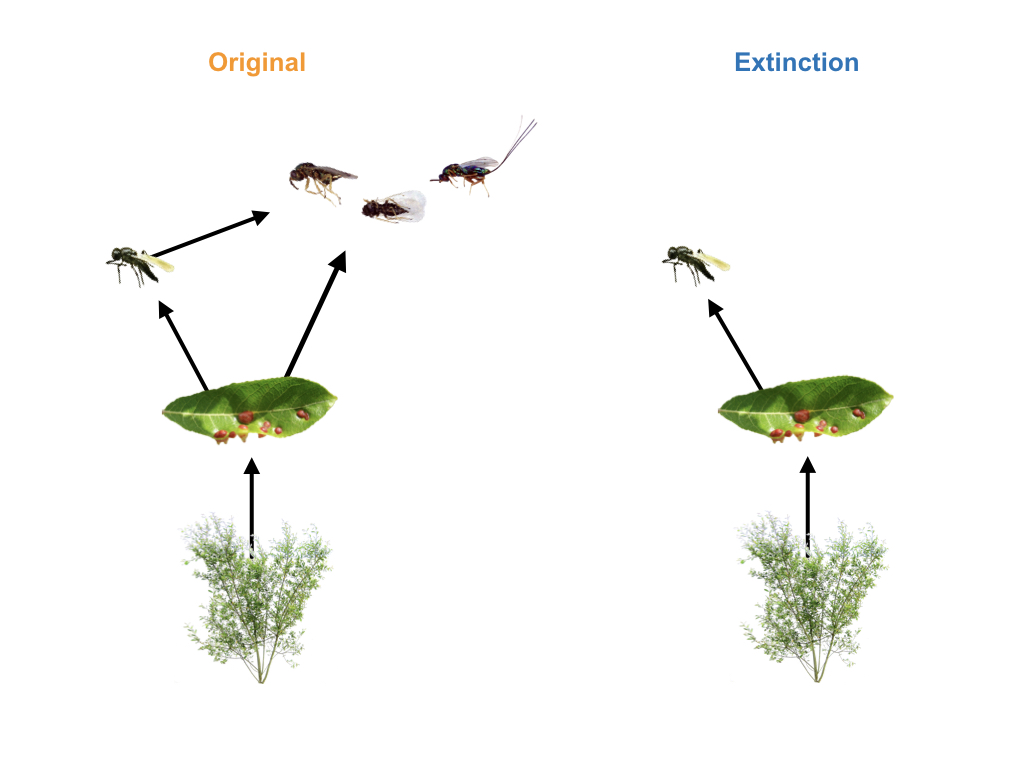
\includegraphics{../analyses/complex_simple_foodwebs_v3.jpeg}
\caption{\label{fig:Conceptual}Experimental manipulation of food-web
structure associated with a leaf-galling midge (\emph{Iteomyia
salicisverruca}) feeding on the willow \emph{Salix hookeriana}. Black
arrows denote the flow of energy in this network of trophic
interactions. In the original food web, we allowed the full suite of egg
and larval parasitoids to impose selection. To simulate consumer
extinction, we used mesh bags to exclude the guild of larval
parasitoids, only allowing the egg parasitoid (\emph{Platygaster} sp.)
to impose selection. Larval parasitoids include the following species
(from left to right): \emph{Mesopolobus} sp. (Family: Pteromalidae);
\emph{Tetrastichus} sp. (Family: Eulophidae); and \emph{Torymus} sp.
(Family: Torymidae).}
\end{figure}

\section{Methods}\label{methods}

\subsection{Study Site}\label{study-site}

We conducted our study within a four-year old common garden experiment
of coastal willow (\emph{Salix hookeriana}) located at Humboldt Bay
National Wildlife Refuge (HBNWR) (40 40'53``N, 124 12'4''W) near Loleta,
California, USA. This common garden consists of 26 different willow
genotypes that were collected from a single population of willows
growing around Humboldt Bay. Stem cuttings of each genotype (25
replicates per genotype) were planted in a completely randomized design
in two hectares of a former cattle pasture at HBNWR. Willows at our
study site begin flowering in February and reach their peak growth in
early August. During this study, willows had reached 5 - 9m in height.
Further details on the genotyping and planting of the common garden are
available in \citet{Barbour2015}.

\subsection{Manipulating Food-web
Structure}\label{manipulating-food-web-structure}

We setup our food-web manipulation across 128 plants soon after galls
began developing on willows in early June of 2013. These 128 plants came
from eight different plant genotypes that spanned the range of trait
variation observed in this willow population \citep{Barbour2015}. For
the original food web (eight replicates per genotype), we used flagging
tape to mark 14 galled leaves per plant (\textasciitilde{}30 larvae),
allowing the full suite of egg and larval parasitoids to impose
selection. Marking galls with flagging tape ensured that all galls had
similar phenology when we collected galls later in the season. To
simulate consumer extinctions, we enclosed 14 galled leaves with 10x15cm
organza bags (ULINE, Pleasant Prairie, WI, USA) to exclude three
parasitoid species that attack during larval development. This treatment
did not exclude the egg parasitoid \emph{Platygaster} sp., which attacks
prior to gall initiation \citep[larva initiate gall development in
Cecidomyiid midges:][]{Gagne1989}. In late August, we collected marked
and bagged galls from each plant, placed them into 30 mL vials and kept
them in the lab for 4 months at room temperature. We then opened galls
under a dissecting scope and determined whether larvae survived to
pupation (our measure of fitness) or were parasitized. We did not
include other sources of mortality, such as early larval death, as they
could influence the expression of the gall phenotype and confound
estimates of selection. For the food-web treatment that excluded larval
parasitoids, we further restricted our data by removing any incidental
instances of parasitism by a larval parasitoid. This represented less
than 3\% of the observations in this food-web treatment and allowed us
to focus our inferences of selection on those imposed by the egg
parasitoid. Our final dataset contains survival estimates for 1285
larvae from 613 galls and 111 plants.

\subsection{Measuring Phenotypic
Traits}\label{measuring-phenotypic-traits}

We collected data on three different traits that we expected to
influence larval survival based on previous work in this system
\citep{Barbour2016} and other work with gall midges
\citep{Weis1983, Heath2018}. First, we measured gall diameter as the
size of each gall chamber to the nearest 0.01 mm at its maximum diameter
(perpendicular to the direction of plant tissue growth). Previous work
in this system has shown that larger galls are associated with higher
survival \citep{Barbour2016}. Second, we measured clutch size by
counting the number of chambers in each gall
\citep{Weis1983, Heath2018}. All larvae collected from the same
multi-chambered gall were scored with the same clutch size. Third, we
measured oviposition preference as the density of larvae observed on a
plant in an independent survey. We did this by randomly sampling five
branches per tree and counting the number of individual gall chambers
(number of larvae). We then converted these counts to a measure of
larval density per 100 shoots by counting the number of shoots on the
last branch we sampled. All larvae collected from the same plant were
scored with the same oviposition preference. Measuring larval densities
on plants in the field is a common method for measuring oviposition
preference \citep{Gripenberg2010}; however, caution must be taken in
inferring `preference' as larval densities can be influenced by
processes other than preference \citep{Singer1986}. Fortunately, a
couple features of our study system suggest that larval densities may be
a good proxy for oviposition preference. For example, since our data
comes from a randomized placement of plant genotypes in a common garden,
there is no consistent bias in which plant genotypes females are exposed
to while searching for oviposition sites. Also, egg predation is a minor
source of mortality for galling insects in general \citep{Hawkins1997};
therefore, we do not expect any prior egg predation to bias our
estimates of observed larval densities.

\subsection{Quantifying the Adaptive
Landscape}\label{quantifying-the-adaptive-landscape}

Inferring adaptive landscapes assumes that trait distributions are
multivariate normal \citep{Lande1983}. To approximate this assumption,
we log-transformed clutch size and square-root transformed oviposition
preference. We then scaled all phenotypic traits (mean=0 and SD=1) prior
to our analyses (detailed below) to ensure that our estimates of
selection were comparable across traits and with other studies.

Our analysis consisted of three parts. First, we used generalized linear
mixed models (GLMM) to quantify selection surfaces \textemdash linear
and nonlinear relationships between absolute fitness (\(W\)) and
standardized phenotypic traits (\(i\)) of individuals \textemdash in
each food-web treatment. Second, we translated selection surfaces into
the scale of relative fitness (\(w\)) in order to calculate standardized
selection gradients. Third, we used our estimates of selection gradients
to characterize the slope and curvature of the adaptive landscape, which
we used to measure evolutionary constraints.

\textbf{Selection surfaces}: Since larval survival was our measure of
absolute fitness, we used a GLMM that assumed a binomial error
distribution (and logit-link function). To approximate the selection
surface, we modelled larval survival as a function of food-web treatment
as well as linear (\(\alpha_i\)), quadratic (\(\alpha_{ii}\)), and
linear interactions (\(\alpha_{ij}\)) between each trait. We also
allowed these selection surfaces (\(\alpha\)) to vary between food-web
treatments. Note that to obtain valid estimates of linear selection
surfaces, we removed nonlinear terms prior to estimating linear
relationships \citep{Lande1983}. Other approaches have been advocated
for approximating selection surfaces \citep{Schluter1988}; however, our
approach enables us to calculate selection gradients, and thus is more
appropriate for approximating the adaptive landscape \citep{Arnold2003}.
To account for the nonindependence of clutch size (measured at gall
level) and oviposition preference (measured at plant level) as well as
any independent effects of willow genotype on larval survival, we
modelled gall ID nested within plant ID nested within genotype ID as
random effects. Although statistical models with random effects are not
common in analyses of natural selection, we think that modelling random
effects can mitigate biased estimates of selection due to environmental
covariances between traits and fitness \citep{Rausher1992}. Since our
end goal was to characterize the relationship between mean trait values
and mean fitness (adaptive landscape), we assumed the mean value of our
random effects (i.e., setting them to zero) when calculating selection
surfaces. We then used parametric bootstrapping (1,000 replicates) to
estimate the effect of food-web treatment on larval survival as well as
selection surfaces in each food-web treatment.

\textbf{Selection gradients}: Selection gradients cannot be estimated
directly from GLMMs of selection surfaces because the response is in
terms of absolute fitness and the coefficients are on a nonlinear scale.
For example, the coefficients in the above model measure the change in
the logarithm of the odds of surviving (i.e.,
\(\text{ln}\{W(z)/[1-W(z)]\}\)) associated with 1 SD change in a trait
with all other traits held fixed at their mean. Therefore, we used the
method developed by \citet{Janzen1998} to translate selection surfaces
from the above model into the scale of relative fitness in order to
calculate directional (\(\beta_i\)), quadratic (\(\gamma_{ii}\)), and
correlational (\(\gamma_{ij}\)) selection gradients. Briefly, this
method calculates the average gradient of selection surfaces by
multiplying the average of \(W(z)[1-W(z)]\) by each regression
coefficient (e.g. \(\alpha_i\), \(\alpha_{ii}\), or \(\alpha_{ij}\)). We
then divided this average gradient by the mean fitness (\(\bar W\)) to
put it on the scale of relative fitness, and thus interpretable as a
selection gradient. We estimated selection gradients separately for each
food-web treatment. Note that we doubled all quadratic terms prior to
calculating selection gradients to put them on the same scale as
estimates of directional and correlational selection
\citep{Stinchcombe2008}.

\textbf{Evolutionary constraints}: We measured evolutionary constraints
by inspecting the slope and curvature of the adaptive landscape. The
number of selective constraints is determined by the slope of the
adaptive landscape, which in our study corresponds to:

\[\textbf{Slope} = \begin{pmatrix} \beta_{\text{Diam}} \\ \beta_{\text{Clutch}} \\ \beta_{\text{Pref}} \end{pmatrix} \]
where each \(\beta_i\) corresponds to the directional selection gradient
acting on each trait. By comparing the number of directional selection
gradients that show clear evidence of contributing to the slope (i.e.,
95\% CI does not overlap zero) in our food-web treatments, we can infer
the effect of food-web structure on selective constraints.

The indirect effects of selection on the G-matrix
(\(\Delta\text{G}=\text{G}(\gamma - \beta \beta^\text{T})\text{G}\)) is
governed by the curvature of the adaptive landscape
(\(\text{C}=\gamma - \beta \beta^\text{T}\)), which in our study
corresponds to:

\[\textbf{Curvature} = \begin{pmatrix} \gamma_{\text{Diam:Diam}}&& \\ \gamma_{\text{Clutch:Diam}}&\gamma_{\text{Clutch:Clutch}}& \\ \gamma_{\text{Pref:Diam}} & \gamma_{\text{Pref:Clutch}} &\gamma_{\text{Pref:Pref}} \end{pmatrix} - \begin{pmatrix} \beta_{\text{Diam}}\beta_{\text{Diam}}&& \\ \beta_{\text{Clutch}}\beta_{\text{Diam}}&\beta_{\text{Clutch}}\beta_{\text{Clutch}}& \\ \beta_{\text{Pref}}\beta_{\text{Diam}} & \beta_{\text{Pref}}\beta_{\text{Clutch}} &\beta_{\text{Pref}}\beta_{\text{Pref}} \end{pmatrix}\]

where each \(\gamma_{ii}\) (diagonal) corresponds to the quadratic
selection gradient acting on a trait, and each \(\gamma_{ij}\)
(off-diagonal) corresponds to the correlational selection gradient
acting on a particular trait combination. Note that we ommitted the
upper triangle of each matrix for clarity since it is simply the
reflection of the lower triangle. Subtracting these two matrices results
in the curvature matrix of the adaptive landscape:

\[\textbf{Curvature} = \begin{pmatrix} \text{C}_{\text{Diam:Diam}}&& \\ \text{C}_{\text{Clutch:Diam}} & \text{C}_{\text{Clutch:Clutch}} & \\ \text{C}_{\text{Pref:Diam}} & \text{C}_{\text{Pref:Clutch}} & \text{C}_{\text{Pref:Pref}} \end{pmatrix}\]
where each \(\text{C}_{ii}\) (diagonal) represents the effect of
selection on the additive genetic variance in a trait, and each
\(\text{C}_{ij}\) (off-diagonal) represents the effect of selection on
the additive genetic covariance between a particular trait combination.
In other words, the sign of diagonal terms of the curvature matrix
dictate whether selection will increase (+), decrease (-), or cause no
change (0) in the additive genetic variance of a trait. Similarly, any
nonzero covariance terms (off-diagonal) are indicative of selection for
trait integration (i.e., less independence). Therefore, we can infer the
number of genetic constraints by summing the number of negative signs
along the diagonal (decrease in additive genetic variance) and the
number of nonzero terms along the off-diagonal (trait integration) of
the curvature matrix. For these analyses, we retained estimates for
selection gradients that showed clear evidence of being different from
zero (i.e., 95\% CI did not overlap zero) and set other gradients to
zero, prior to calculating the curvature matrix in each food-web
treatment. This provides a conservative estimate of the factors
contributing to the curvature of the adaptive landscape.

Note that our metrics of selective and genetic constraints do not put
much stock in differences in the magnitude of selection between food-web
treatments. This is because there is a high likelihood that we are
underestimating the magnitude of selection in our treatment that
excludes larval parasitoids. We expect this because larval parasitoids
not only impose mortality on gall midges, but egg parasitoids as well
(fig. \ref{fig:Conceptual}). Therefore, our short-term removal of larval
parasitoids has not allowed for an increase in egg parasitoid abundance
after being released from intraguild predation. An increase in the
abundance of egg parasitoids would decrease mean survival of gall
midges, thus increasing the variance in relative fitness of midges, and
consequently the magnitude of selection estimates. A recent paper by
\citet{Hunter2018} highlights this pervasive effect of survival on the
magnitude of selection estimates. This is why we use more qualitative
metrics of evolutionary constraints (i.e., selective constraints =
number of traits under directional selection; genetic constraints =
number of decreasing variances + nonzero covariances).

\subsection{Adjusting for biased measurements of
selection}\label{adjusting-for-biased-measurements-of-selection}

Rather than imposing selection, parasitoids may influence the expression
of herbivore traits which could bias measurements of selection. In our
system, it was plausible that parasitoids may influence chamber diameter
by altering larval feeding behavior or killing larvae before they
complete their development. To estimate this potential bias, we subset
our data to only include galls where there was variation in larval
survival within the same gall (i.e.~1 \textgreater{} mean survival
\textgreater{} 0). If we assume that larvae within each gall should have
similar chamber diameters because they come from the same clutch and
experience the same local environment (an assumption our data supports:
gall ID explains 54\% of the variance in chamber diameter), then the
relationship between chamber diameter and larval survival in this data
subset represents the effect of parasitism on trait expression
(i.e.~bias). We used a GLMM with the same structure as described above
except that we modeled only a linear relationship between chamber
diameter and larval survival (\(\alpha_{\text{Diam}}\)). We detected a
positive bias in both food-web treatments (original
\(\alpha_{\text{Diam}}\)= 0.36 {[}0.05, 0.67{]}; extinction
\(\alpha_{\text{Diam}}\)= 0.42 {[}0.01, 0.82{]}), indicating that
unadjusted relationships would overestimate the strength of selection on
chamber diameter. To account for this bias, we substracted our mean
estimates of bias from our estimates with the full dataset prior to
calculating chamber diameter's selection surface and directional
selection gradient.

\subsection{Measuring selection on egg
parasitoids}\label{measuring-selection-on-egg-parasitoids}

Once parasitized, the gall phenotype becomes the phenotype of the egg
parasitoid. This phenotype may influence the egg parasitoid's survival
in the face of larval parasitoids, and thus experiences selection. Our
food-web manipulation allows us to measure selection imposed by larval
parasitoids on the phenotype of egg parasitoids. Using the same models
as described above, we substituted egg parasitism as our response
variable to quantify selection surfaces and selection gradients acting
on the egg parasitoid. Note that we cannot test the effect of food-web
structure on the egg parasitoid's adaptive landscape ---we can only
estimate selection imposed by larval parasitoids. This comparison is
still useful though in determining the extent to which the community
context may have indirect evolutionary effects by altering selection on
multiple interacting populations.

All analyses and visualizations were conducted in R \citep{R2018}.
Unless otherwise noted, we report mean estimates of selection surfaces
and selection gradients with 95\% confidence intervals in brackets. Note
that for visualizing the adaptive landscape we restrict trait axes to
\(\pm 1\) SD of the mean trait value. This emphasizes the fact that we
can only reliably estimate the shape of the adaptive landscape near the
mean phenotype of the population \citep{Arnold2001}. We also plot mean
larval survival on a natural log scale to accurately reflect the
mathematical definition of the adaptive landscape \citep{Arnold2003}.
All data and code to reproduce the reported results are publicly
available on GitHub and have been archived on Zenodo (links are
available from the journal office).

\section{Results}\label{results}

\subsection{Consumer extinctions increase selective
constraints}\label{consumer-extinctions-increase-selective-constraints}

\indent We found that the extinction of larval parasitoids increased the
number of gall midge traits under directional selection (3 of 3)
relative to the original food web (1 of 3)(table \ref{Table:Gradients}).
For example, we observed directional selection for smaller clutch sizes
when we excluded larval parasitoids, but there was no evidence of
selection acting on this trait in the original food web (table
\ref{Table:Gradients}; fig. \ref{fig:UV_Landscape}C). This absence of
selection appeared to be a result of conflicting selection pressures
imposed by each guild of parasitoids. Specifically, when we subset our
data to focus on differences between parasitoid guilds, we found that
larval parasitoids actually impose directional selection for larger
clutch sizes (\(\beta_{\text{Clutch}}\)= 0.13 {[}0.04, 0.24{]}). We also
observed clear evidence of directional selection for midges to avoid
ovipositing on plants with high densities of conspecifics when we
excluded larval parasitoids (table \ref{Table:Gradients}; fig.
\ref{fig:UV_Landscape}B); however, there was no clear relationship in
the original food web (table \ref{Table:Gradients}). This was likely a
result of larval parasitoids imposing greater mortality on egg
parasitoids at high gall midge densities (see Selection on egg
parasitoids section), and thus a less than additive effect on gall
midges. Chamber diameter experienced positive directional selection in
both food-web treatments (fig. \ref{fig:UV_Landscape}A). Although the
magnitude of selection on chamber diameter was relatively higher in the
original food web (table \ref{Table:Gradients}), this was not due to any
difference in the relationship between chamber diameter and survival
(selection surfaces: original \(\alpha_{\text{Diam}}\)= 1.15 {[}0.75,
1.61{]}; extinction \(\alpha_{\text{Diam}}\)= 1.1 {[}0.64, 1.65{]}), but
was simply a consequence of the (expected) lower survival in the
original food web (original \(\bar W\)= 0.42 {[}0.28, 0.56{]};
extinction \(\bar W\)= 0.68 {[}0.54, 0.81{]}).

\bigskip

\begin{table}[h]
\caption{Standardized selection gradients acting on gall midges in the original food web and with the extinction of larval parasitoids.}
\label{Table:Gradients}
\centering
\begin{tabular}{lcc} %c
\\ 
\hline
\textbf{Selection gradient} & \textbf{Original} & \textbf{Extinction}   \\ %& \textbf{Contrast}
\hline
$\beta_{\text{Diam}}$ & 
\textbf{
0.34 [
0.22,
0.48] }& 
\textbf{
0.21 [
0.12,
0.31] }\\%& 
%\textbf{
%0.14 [
%0.27,
%0] }\\

$\beta_{\text{Clutch}}$ & 
0.06 [
-0.05,
0.17] & 
\textbf{
-0.09 [
-0.17,
-0.01] }\\%& 
%\textbf{
%0.15 [
%0.29,
%0.03] }\\

$\beta_{\text{Pref}}$ &
-0.13 [
-0.29,
0.05] & 
\textbf{
-0.16 [
-0.26,
-0.06] }\\%& 

%0.03 [
%0.21,
%-0.15] \\

$\gamma_{\text{Diam:Diam}}$ &
0.13 [
-0.06,
0.33] & 

0.1 [
-0.02,
0.23] \\%& 

%0.03 [
%0.27,
%-0.2] \\

$\gamma_{\text{Clutch:Clutch}}$ & 
-0.05 [
-0.27,
0.18] & 

-0.11 [
-0.28,
0.03] \\%& 

%0.06 [
%0.32,
%-0.2] \\

$\gamma_{\text{Pref:Pref}}$ & 
\textbf{
0.34 [
0.07,
0.63] }& 

0.02 [
-0.15,
0.18] \\%& 
%\textbf{
%0.32 [
%0.64,
%0.01] }\\

$\gamma_{\text{Diam:Clutch}}$ & 
-0.04 [
-0.16,
0.08] & 

-0.07 [
-0.15,
0.02] \\%& 

%0.02 [
%0.17,
%-0.12] \\

$\gamma_{\text{Diam:Pref}}$ & 
-0.13 [
-0.29,
0.02] & 

-0.02 [
-0.1,
0.07] \\%& 

%-0.12 [
%0.05,
%-0.3] \\

$\gamma_{\text{Clutch:Pref}}$ & 
0.03 [
-0.1,
0.18] & 

0 [
-0.07,
0.07] \\%& 

%0.03 [
%0.18,
%-0.12] \\ 
\hline
\end{tabular}
\bigskip{}
\\
{\footnotesize Note: Values in brackets represent 95\% confidence intervals. Bold values indicate that the 95\% CI does not overlap zero. $\beta_{\text{Diam}}$ has been adjusted for bias.}
\end{table}

\subsection{Consumer extinctions increase genetic
constraints}\label{consumer-extinctions-increase-genetic-constraints}

\indent The curvature of the adaptive landscape indirectly affects
genetic constraints and is influenced by directional, quadratic, and
correlational selection gradients. There was no clear evidence of
correlational selection for any combination of traits in either food-web
treatment (table \ref{Table:Gradients}). Similarly, there was no clear
evidence of quadratic selection on chamber diameter or clutch size in
either food-web treatment (table \ref{Table:Gradients}; fig.
\ref{fig:UV_Landscape}A,C). In contrast, our food-web treatment did
alter quadratic selection acting on oviposition preference (table
\ref{Table:Gradients}). The negative relationship between oviposition
preference and larval survival dampened at high densities in the
original food web, but not with the exclusion of larval parasitoids
(fig. \ref{fig:UV_Landscape}B). This dampened relationship was partly
due to a trend for nonlinear selection imposed by larval parasitoids
(\(\gamma_{\text{Pref:Pref}}\)= 0.18 {[}-0.02, 0.42{]}), but was also
magnified by the lower average survival in complex food webs.

\begin{figure}
\centering
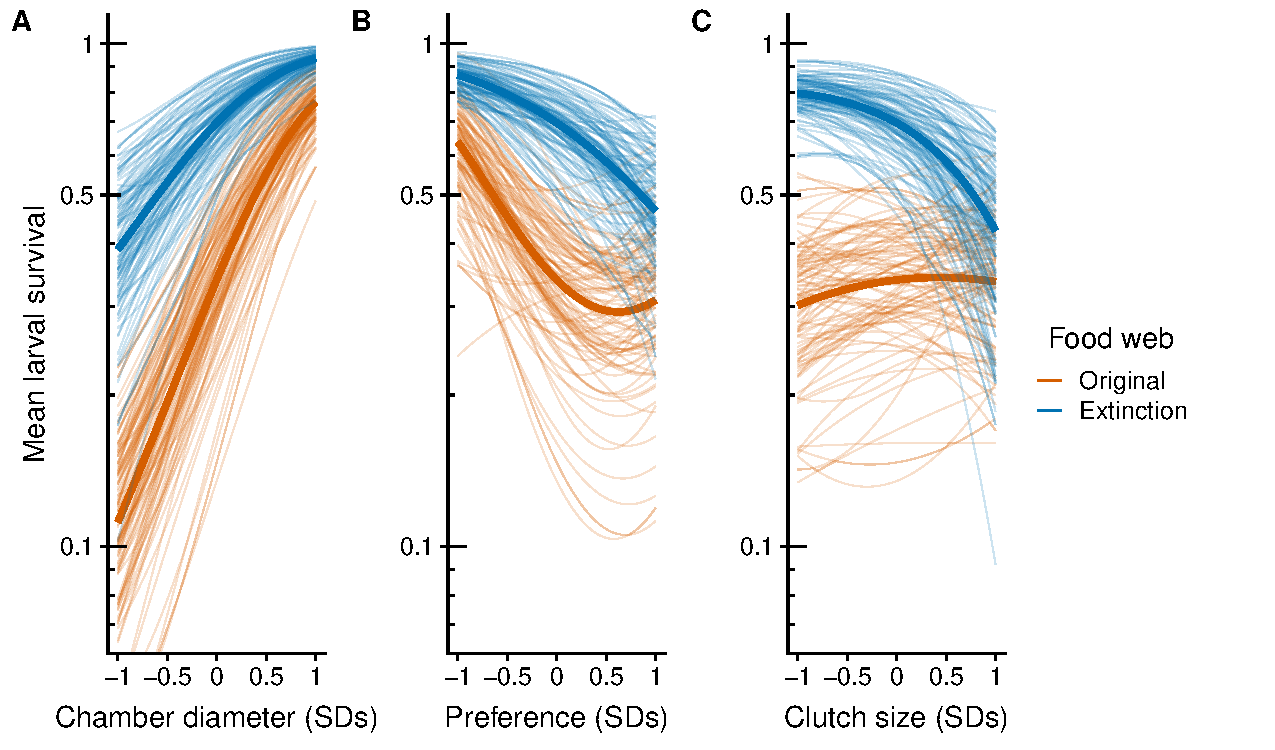
\includegraphics{../analyses/UV_landscapes.pdf}
\caption{\label{fig:UV_Landscape}Adaptive landscape of gall midge
phenotypes in the original food web and with the extinction of larval
parasitoids. Each panel corresponds to a different phenotypic trait:
chamber diameter (A); oviposition preference (B); and clutch size (C).
Bold lines represent selection experienced in the original food web
(orange) and with consumer extinctions (blue). Thin lines represent
bootstrapped replicates to show the uncertainty in selection. For
clarity, we only display 100 bootstraps even though inferences are based
on 1,000 replicates. Note that mean larval survival is plotted on a
natural log scale to reflect the mathematical defintion of the adaptive
landscape.}
\end{figure}

Using our estimates of directional (\(\beta_i\)), quadratic
(\(\gamma_{ii}\)), and correlation selection (\(\gamma_{ij}\)), we
calculated the curvature (\(\text{C}=\gamma - \beta \beta^\text{T}\)) of
the adaptive landscape in each food-web treatment. In our study, this
corresponds to:

\[\textbf{Curvature} = \begin{pmatrix} \gamma_{\text{Diam:Diam}}&& \\ \gamma_{\text{Clutch:Diam}}&\gamma_{\text{Clutch:Clutch}}& \\ \gamma_{\text{Pref:Diam}} & \gamma_{\text{Pref:Clutch}} &\gamma_{\text{Pref:Pref}} \end{pmatrix} - \begin{pmatrix} \beta_{\text{Diam}}\beta_{\text{Diam}}&& \\ \beta_{\text{Clutch}}\beta_{\text{Diam}}&\beta_{\text{Clutch}}\beta_{\text{Clutch}}& \\ \beta_{\text{Pref}}\beta_{\text{Diam}} & \beta_{\text{Pref}}\beta_{\text{Clutch}} &\beta_{\text{Pref}}\beta_{\text{Pref}} \end{pmatrix}\]

\[\textbf{Curvature} = \begin{pmatrix} \text{C}_{\text{Diam:Diam}}&& \\ \text{C}_{\text{Clutch:Diam}} & \text{C}_{\text{Clutch:Clutch}} & \\ \text{C}_{\text{Pref:Diam}} & \text{C}_{\text{Pref:Clutch}} & \text{C}_{\text{Pref:Pref}} \end{pmatrix}\]
\bigskip

where each \(\text{C}_{ii}\) (diagonal) represents the effect of
selection on the additive genetic variance in a trait, and each
\(\text{C}_{ij}\) (off-diagonal) represents the effect of selection on
the additive genetic covariance between a particular trait combination.
In order to obtain a conservative estimate of the factors contributing
to the curvature, we only used estimates of selection that clearly
differed from zero (bold values in table \ref{Table:Gradients}),
otherwise we set estimates of selection to zero (non-bold values in
table \ref{Table:Gradients}) prior to our calculation. We found that the
curvatures of the adaptive landscape exhibited the following structures:

\[\textbf{Curvature}_{\text{original}} = \begin{pmatrix} 
0 &  &  \\  
0 & 0 &  \\  
0 & 0 & 0.34 \end{pmatrix} - \begin{pmatrix} 
0.34\cdot0.34 &  &  \\  
0\cdot0.34 & 0\cdot0 &  \\  
0\cdot0.34 & 0\cdot0 & 0\cdot0 \end{pmatrix}\]

\[\textbf{Curvature}_{\text{original}} = \begin{pmatrix} 
-0.12 &  &  \\  
0 & 0 &  \\  
0 & 0 & 0.34 \end{pmatrix}\]

\[\textbf{Curvature}_{\text{extinction}} = \begin{pmatrix} 
0 &  &  \\  
0 & 0 &  \\  
0 & 0 & 0 \end{pmatrix} - \begin{pmatrix} 
0.21\cdot0.21 &  &  \\  
-0.09\cdot0.21 & -0.09\cdot-0.09 &  \\  
-0.16\cdot0.21 & -0.16\cdot-0.09 & -0.16\cdot-0.16 \end{pmatrix}\]

\[\textbf{Curvature}_{\text{extinction}} = \begin{pmatrix} 
-0.04 &  &  \\  
0.02 & -0.01 &  \\  
0.03 & -0.01 & -0.03 \end{pmatrix}\]

Remember that we can infer the indirect effects of selection on genetic
constraints by summing the number of negative signs along the diagonal
(decrease in additive genetic variance) and the number of nonzero terms
along the off-diagonal (trait integration) of the curvature matrix. The
structure of these matrices indicates that the extinction of larval
parasitoids increased the number of genetic constraints on gall midges
(6 of 6) relative to the original food web (1 of 6). For example,
directional selection resulting from the exclusion of larval parasitoids
acted to decrease genetic variance for all three phenotypic traits
(negative diagonal terms), whereas only one trait (chamber diameter)
experienced a decrease in additive genetic variance in the original food
web. For genetic covariances, the combined effects of directional
selection resulting from consumer extinctions favored integration among
all three phenotypic traits (nonzero off-diagonal terms), and thus
constraints along all three axes of covariance (fig.
\ref{fig:MV_Landscape}). In contrast, the absence of directional
selection in clutch size and oviposition preference did not promote
trait integration along any axis in the original food web (fig.
\ref{fig:MV_Landscape}).

\begin{figure}
\centering
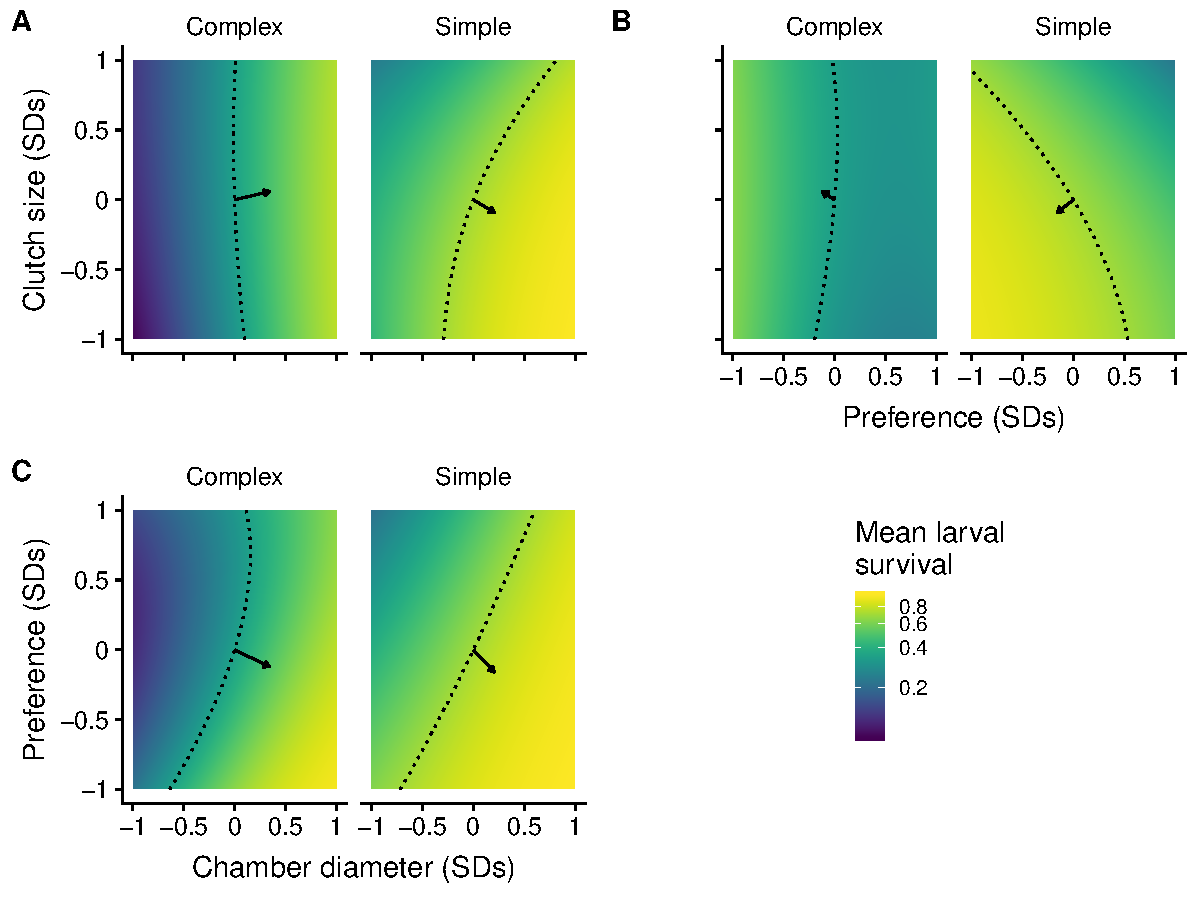
\includegraphics{../analyses/MV_landscapes.pdf}
\caption{\label{fig:MV_Landscape}Two dimensional view of adaptive
landscapes of gall midge phenotypes in the original food web and with
the extinction of larval parasitoids. Each panel corresponds to a
different combination of phenotypic traits: clutch size and chamber
diameter (A); clutch size and oviposition preference (B); oviposition
preference and chamber diameter (C). Arrows represent mean estimates of
directional selection gradients, while contours represent predicted
larval survival of the mean phenotype in each food-web treatment. Notice
that arrows point more toward a corner of the adaptive landscape for
each combination of traits with the extinction of larval parasitoids
compared to the original food web. This indicates that consumer
extinctions more strongly favored trait integration (covariance). Note
that mean larval survival is plotted on a natural log scale to reflect
the mathematical definition of the adaptive landscape.}
\end{figure}

\subsection{Selection on egg
parasitoids}\label{selection-on-egg-parasitoids}

The extinction of larval parasitoids only altered the relationship
between gall midge preference and the probability of observing egg
parasitoids (table \ref{Table:ExtendedGradients}). Specifically, the
impact of larval parasitoids increased nonlinearly with higher gall
midge densities (fig. \ref{fig:EggPtoid_Selection}).

\bigskip

\begin{table}[h]
\caption{Standardized selection gradients acting on egg parasitoids (\textit{Platygaster} sp.)}
\label{Table:ExtendedGradients}
\centering
\begin{tabular}{lc}
\\ 
\hline
\textbf{Selection gradient} & \textbf{Contrast = Original - Extinction}  \\ 
\hline
$\beta_{\text{Diam}}$ & 

-0.03 [
-0.3,
0.25] \\

$\beta_{\text{Clutch}}$ & 

0.07 [
-0.26,
0.39] \\

$\beta_{\text{Pref}}$ &

-0.25 [
-0.64,
0.09] \\

$\gamma_{\text{Diam:Diam}}$ &

-0.05 [
-0.43,
0.33] \\

$\gamma_{\text{Clutch:Clutch}}$ & 

-0.21 [
-0.68,
0.26] \\

$\gamma_{\text{Pref:Pref}}$ & 

\textbf{
-0.46 [
-1.07,
-0.02] }\\

$\gamma_{\text{Diam:Clutch}}$ & 

0 [
-0.29,
0.27] \\

$\gamma_{\text{Diam:Pref}}$ & 

0.25 [
-0.04,
0.6] \\

$\gamma_{\text{Clutch:Pref}}$ & 

-0.18 [
-0.52,
0.12] \\ 
\hline
\end{tabular}
\bigskip{}
\\
{\footnotesize Note: Values in brackets represent 95\% confidence intervals. Bold values indicate that the 95\% CI does not overlap zero. $\beta_{\text{Diam}}$ has been adjusted for bias.}
\end{table}

\begin{figure}
\centering
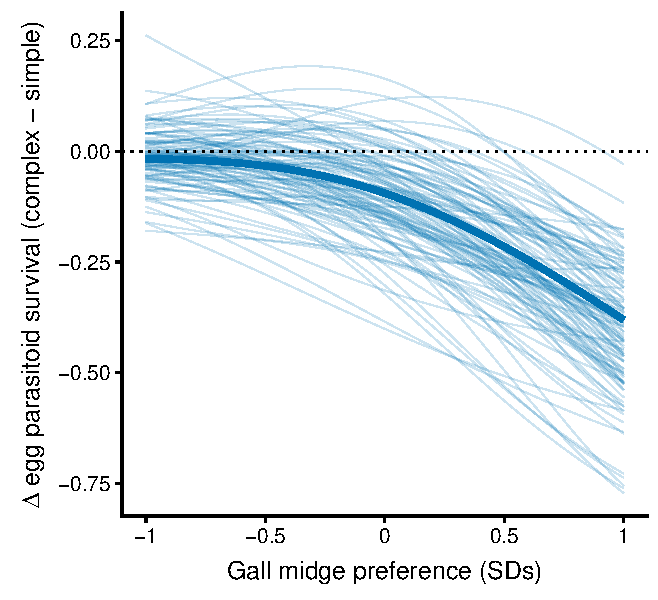
\includegraphics{../analyses/selection_on_Platygaster.pdf}
\caption{\label{fig:EggPtoid_Selection}Selection imposed by larval
parasitoids on egg parasitoids (\emph{Platygaster} sp.). The bold line
represents the average difference in the probability of observing the
egg parasitoid (original - extinction of larval parastioids) as a
function of gall midge oviposition preference. Thin lines represent
bootstrapped replicates to show the uncertainty in selection. For
clarity, we only display 100 bootstraps even though inferences are based
on 1,000 replicates. The decrease in the probability of observing egg
parasitoids at high gall-midge densities indicate that larval
parasitoids impose nonlinear selection on egg parasitoids.}
\end{figure}

\section{Discussion}\label{discussion}

We found that the extinction of larval parasitoids constrained
phenotypic evolution in gall midges in two key ways. First, more traits
contributed to the slope of the adaptive landscape in the absence of
larval parasitoids, suggesting greater constraints on the trajectory of
phenotypic evolution. Second, excluding larval parasitoids indirectly
increased the number of genetic constraints, which could act to
constrain the gall midge's adaptive potential in the face of novel
selection pressures. Our experiment also revealed evidence of indirect
selection pressures, suggesting that the loss of consumers may have
complex effects on the trajectories of phenotypic evolution. Taken
together, our study provides experimental evidence from the field that
consumer extinctions may constrain the adaptive potential of remaining
populations.

All three phenotypic traits we examined experienced directional
selection when we excluded larval parasitoids, indicating that there is
an optimal phenotype that maximizes larval survival (i.e.~large chamber
diameter, small clutch size, and avoidance of conspecifics). In
contrast, we did not observe clear evidence of selective constraints on
clutch size and oviposition preference in the original food web. This
suggests that there are many optimal phenotypes (adaptive peaks), or in
this case, a flat adaptive landscape where there are no fitness
consequences for phenotypic change in these traits. This also implies
that as selective constraints dampen in more complex food webs, then the
trajectory of evolution becomes more determined by how genetic
constraints interact with other evolutionary processes (e.g.~genetic
drift, gene flow, and mutation). Interestingly, this aligns with
\citet{Schluter1996}`s hypothesis that phenotypic evolution often
follows 'genetic lines of least resistance'. \citet{Schluter1996} found
support for this hypothesis from data on natural populations of several
vertebrate species, including threespine sticklebacks, a few species of
songbirds, and mice from the genus \emph{Peromyscus}. All of these
species occupy intermediate trophic levels and are likely embedded in
complex food webs, which is consistent with our suggestion that genetic
constraints may have a stronger influence in more complex food webs.

We also found evidence for more genetic constraints when we excluded
larval parasitoids due to indirect effects of selection on the
population's G-matrix. The ability of a population to adapt to novel
selection pressures (evolvability) is largely governed by the structure
of its G-matrix \citep{Hansen2008}. When selection favors genetic
covariance between traits (positive or negative), this results in less
autonomy of evolutionary responses to changing environments. Similarly,
decreases in genetic variance constrain potential for the trait itself
to evolve. Together, this suggests that consumer extinctions may
decrease the evolutionary potential of populations by indirectly
selecting for decreases in genetic variance in multiple traits and
favoring trait integration. Current theory often assumes genetic
variances and covariances remain constant over time rather than
dynamically changing with the community context
\citep{McPeek2017, Guimaraes2017}. Our empirical results highlight the
need to explore the evolutionary consequences of not only direct effects
of selection, but indirect effects on genetic constraints that are
shaped by the community context.

The generality of our results likely depends on the relative abundance
and functional differences between consumers in a community. For
example, if consumers do not differ from each other, then we do not
expect changes in food-web structure to modify evolutionary constraints.
Also, many consumers may be at too low of abundances to impose selection
on their resources. Rank abundance curves \citep{Preston1948} and the
disproportionate number of weak interactions in diverse communities
\citep{Paine1992} support this notion. When consumers are abundant
though, the effect of food-web structure will depend on whether
different species impose conflicting selection pressures or select for
distinct traits. For example, parisitoids and birds impose conflicting
selection pressures on the size of galls induced by the fly
\emph{Eurosta solidaginis} \citep{Weis1985, Abrahamson1997}. Recent
studies in this system have shown that decreases in the relative
abundance of birds, due to either small patch sizes \citep{Start2016} or
proximity to urban areas \citep{Start2018} causes a shift from neutral
to directional selection on gall size. On the other hand, different
consumers may impose selection on different traits, favoring trait
integration and increasing genetic constraints. Examples of this include
strong genetic covariances in plant resistance to different insect
herbivores \citep{Maddox1990, Wise2007, Wise2013}, although there are
also examples where these covariances are weak
\citep{Roche1997, Barbour2015}, or vary from year-to-year
\citep{Johnson2007}. We suggest that gaining predictive insight to the
evolutionary consequences of food-web disassembly requires an
understanding of the mechanisms governing the assembly of trophic
interactions.

Our results suggest that the loss of consumers may not only directly
affect connected species, but also result in indirect evolutionary
effects. In our study, this indirect effect arises from egg parasitoids
being released from intraguild predation when we excluded larval
parasitoids. This release occurs more on trees with high larval
densities, which could intensify selection on gall midge oviposition
preference. A growing number of experiments over the past two decades
have demonstrated the presence and potential importance of indirect
evolutionary effects that emerge in a community context
\citep{Pilson1996, Juenger1998, Stinchcombe2001, Lankau2007, Walsh2008, Walsh2010, terHorst2010, Sahli2011, Lau2012, terHorst2015, Schiestl2018, Start2019}.
If indirect evolutionary effects are common
\citep{Miller1996, Walsh2013}, then predicting evolutionary trajectories
resulting from consumer extinctions will require evolutionary studies to
explicitly account for the ecological networks that species are embedded
in.

There is a growing number of theoretical studies on adaptation to
directional environmental change that incorporate species interactions
\citep[e.g.][]{deMazancourt2008, Johansson2008, Norberg2012, Osmond2017PredatorsHelpPrey}.
This work has given insight to the mechanisms by which pairwise
interactions modify the adaptive potential of species. Our study hints
at a novel mechanism, whereby more complex food webs flatten the
adaptive landscape, thus facilitating future adaptation by allowing
genetic and phenotypic variation to persist. This mechanism only emerges
once we move beyond pairwise interactions to consider selection on
multiple traits in a community context. However, a study on competition
has highlighted that we may expect the opposite effect of species
diversity in competitive communities \citep{deMazancourt2008}. This
negative effect of species diversity on adaptation occurs because there
is a greater chance that the optimal phenotype is already occupied by a
competitor in a more diverse community. More work is needed to examine
how the distribution of different interaction types affects adaptation
to environmental change in species-rich communities.

Our study has some limitations to consider when relating our findings to
the effect of consumer extinctions on evolutionary constraints more
generally. First, we removed other sources of mortality prior to our
analyses. While this was necessary to avoid confounding estimates of
selection with effects on phenotypic expression, we may be
overestimating the effects of selection due to consumers. Second, our
metrics of evolutionary constraints do not account for variation in the
magnitude of selection pressures. While metrics that incorporate the
magnitude of selection are possible \citep{Hansen2008}, they were not
appropriate for our study as our experimental removal of larval
parasitoids artificially increased the mean fitness of gall midges (in
the short term), which dampens the magnitude of selection gradients in
this treatment \citep{Hunter2018}. This is why we used more qualitative
metrics of evolutionary constraints, which are robust to this artificial
effect and simply require sufficient sample sizes to detect evidence of
selection.

Our study gives insight to how consumer extinctions alter evolutionary
constraints on remaining populations. In particular, it hints at a
potential insidious effect of local extinctions that compromises the
robustness of remaining populations to future environmental change. Our
work also highlights some key challenges for predicting phenotypic
evolution in the face of global change. First, the simplification of
ecological communities may actually reduce the predictability of
phenotypic evolution, because knowledge is required of both selective
and genetic constraints, rather than potentially just genetic
constraints in more complex systems. Second, many theoretical models of
eco-evolutionary dynamics focus on phenotypic change in a single trait,
yet our results highlight that the number of traits under selection may
change with the community context. Importantly, we found that different
species/guilds imposed different selection pressures. Knowing these
hidden selection pressures is critical for prediction, because the
trajectory of evolution will depend on the nature of change in the
community context. We expect that a continued integration of adaptive
landscapes and ecological networks will enhance our ability to predict
the evolutionary consequences of changes in ecological communities.

\bibliography{references}


\end{document}
